\documentclass[conference]{IEEEtran}
% EECR official IEEEtran conference format. Reference-reduction revision 2026-11-18.
\IEEEoverridecommandlockouts
\usepackage{cite}
\usepackage{amsmath,amssymb,amsfonts}
\usepackage{algorithmic}
\usepackage{graphicx}
% Keep floats after their source and within their main section. Subsection
% boundaries remain flexible to avoid short columns and large empty spaces.
\usepackage{flafter}
\usepackage[section]{placeins}
\usepackage{balance}
\usepackage{textcomp}
\usepackage[table]{xcolor}
\definecolor{methodblue}{HTML}{2376AC}
\usepackage{url}
\usepackage[hidelinks]{hyperref}
\def\BibTeX{{\rm B\kern-.05em{\sc i\kern-.025em b}\kern-.08em
    T\kern-.1667em\lower.7ex\hbox{E}\kern-.125emX}}

\title{Engineering Minimum-Cost Reach-Avoid Control for Quadruped Navigation}

\author{
  \IEEEauthorblockN{Haoyang Cao}
  \IEEEauthorblockA{\textit{Institute of Software,}\\
  \textit{Chinese Academy of Sciences}\\
  \textit{University of the Chinese}\\
  \textit{Academy of Sciences}\\
  Beijing, China\\
  caohaoyang24@mails.ucas.ac.cn}
  \and
  \IEEEauthorblockN{Yuhua Guo}
  \IEEEauthorblockA{\textit{Space Star Technology Co., Ltd,}\\
  \textit{China Academy of Space Technology}\\
  \textit{State Key Laboratory of Space}\\
  \textit{Information System and Integrated}\\
  \textit{Application, Beijing Institute of}\\
  \textit{Satellite Information Engineering}\\
  Beijing, China\\
  guoyh@radi.ac.cn}
  \and
  \IEEEauthorblockN{Bai Xue}
  \IEEEauthorblockA{\textit{Key Laboratory of}\\
  \textit{System Software}\\
  \textit{Institute of Software,}\\
  \textit{Chinese Academy of Sciences}\\
  Beijing, China\\
  xuebai@ios.ac.cn}
}
% Jingduo Pan was removed from this version at the user's request.
% The remaining author order follows the archived CoRL submission. Haoyang Cao's
% publication-name spelling is corroborated by Bai Xue's team homepage.
% Yuhua Guo's two affiliations follow the author-provided reference images.
% Their shared Beijing address is listed once after both affiliations.
% All authors' Beijing, China locations are confirmed by the user.
% The corresponding author still requires confirmation; do not infer it.

\begin{document}
% Avoid stretching inter-float and heading glue to force equal column bottoms.
\raggedbottom
\maketitle

\begin{abstract}
The deployment of minimum-cost reach-avoid control on a physical quadruped robot is investigated. The challenges of coupled locomotion--navigation learning and model--execution mismatch are addressed through hierarchical control and two data-calibrated margins. Locomotion stabilization is separated from high-level navigation learning by a pretrained, frozen velocity tracker. Before high-level learning, nominal budget accounting is corrected by the cost margin, and the unsafe set is expanded by the geometric margin. Across three navigation scenarios, a success rate of 73.3\% and a budget violation rate of 9.0\% are obtained with the resulting calibrated minimum-cost reach-avoid (CaMRA) system, compared with 70.7\% and 14.0\% for uncalibrated RC-PPO. The distinct roles and deployment limits of these corrections are examined through ablation, held-out calibration, and physical-robot studies. An execution-calibrated pipeline is established to connect nominal minimum-cost reach-avoid planning with quadruped closed-loop execution.
\end{abstract}

\begin{IEEEkeywords}
quadruped navigation, reach-avoid control, safe robot learning
\end{IEEEkeywords}

\section{Introduction}
Quadruped inspection, exploration, and service tasks require collision-free goal
reaching without unnecessary motion or energy expenditure. In cluttered scenes,
short routes may approach obstacles, whereas safer routes may require more time
and actuation. Encoding safety and efficiency as separate reward terms makes
this trade-off depend on hand-tuned weights. Minimum-cost reach-avoid (MCRA)
control instead specifies goal reachability and trajectory-wide avoidance while
minimizing cumulative cost~\cite{bansal2017}.\footnote{The CaMRA implementation
is publicly available at \url{https://github.com/haoyangc2001/NaVILA_CaMRA}.}

Reachability-Constrained Proximal Policy Optimization (RC-PPO)~\cite{so2024}
enables practical MCRA learning by augmenting the state with a safety indicator
and remaining budget, learning a reachability value function and
budget-conditioned policy, and seeking the least feasible initial budget.
These components jointly represent safety and cost feasibility.

Physical deployment also requires translating navigation decisions into joint
motion. Direct joint-level learning must acquire balance and gait coordination
alongside collision-free goal reaching. Encoding falls, excessive body tilt, and
collisions as unsafe states does not fully specify smooth, coordinated locomotion;
early instability may interrupt navigation rollouts and hinder route selection
and cost optimization. We therefore pretrain a velocity tracker for balance,
gait coordination, and action smoothness, freeze it, and learn RC-PPO navigation
through its fixed velocity-command interface.

The tracker improves stability and attenuates disturbances, but identical velocity
commands may still incur extra cost or path deviations, leading to underestimated
budget consumption or overestimated clearance. With the tracker frozen, we pair
nominal and executed rollouts using identical initial conditions and commands.
Empirical cost overruns and path deviations determine a cost margin $\alpha$ and
geometric margin $\delta$, respectively. These increase the running cost in
budget updates and expand the unsafe set before high-level learning and budget
search. Deployment uses the same frozen tracker.

This calibrated minimum-cost reach-avoid (CaMRA) pipeline connects nominal MCRA
learning to physical closed-loop execution. Its scope is empirical robustness
under the calibration execution distribution; we claim neither strict stochastic
safety guarantees nor an extension of RC-PPO's deterministic theory to general
stochastic systems. Controlled mismatch studies, component-wise ablations,
sensitivity tests, and quantitative hardware evaluation assess execution
mismatch, the distinct failure modes addressed by $\alpha$ and $\delta$, and
system behavior on a physical robot.

The main contributions are:
\begin{enumerate}
\item A hierarchical quadruped MCRA framework separates locomotion stabilization
      from navigation learning through a pretrained, frozen velocity tracker,
      providing a consistent calibration and deployment interface.
\item Two margins calibrated from paired nominal and executed trajectories
      separately correct budget accounting and unsafe-set geometry for
      high-level learning and budget selection.
\item Navigation comparisons, ablations, held-out calibration tests, and
      physical-robot evaluation examine both margins' roles and deployment
      trade-offs.
\end{enumerate}

\section{Related Work}
\subsection{Minimum-Cost Reach-Avoid Learning}
Reach-avoid reinforcement learning treats target reaching and unsafe-set
avoidance as trajectory-level requirements rather than competing reward
terms~\cite{bansal2017,hsu2021}. RC-PPO extends this to MCRA through safety/budget
state augmentation, budget-conditioned policy and reachability-critic learning,
and least-feasible-budget search~\cite{so2024}. We adopt this foundation to
connect nominal MCRA decisions to quadruped execution.

\subsection{Safe Quadruped Navigation}
Learned locomotion supports quadruped navigation: Lee et al.~\cite{lee2020}
demonstrated robust natural-terrain locomotion using proprioception. Jin et
al.~\cite{jin2023resilient} trained navigation policies to command an existing
locomotion controller and use locomotion-level observations to respond to
perception failures. He et al.~\cite{he2024abs} instead developed a joint-level
agile policy with reach-avoid-guided switching to collision-avoidance recovery.
Hierarchical policies connect visual navigation and reusable motor
skills~\cite{jain2021pixels}, while iPlanner learns smooth, collision-free paths
from depth observations through differentiable cost maps~\cite{yang2023iplanner}.
Here, a frozen tracker stabilizes locomotion, while high-level MCRA addresses
goal reaching, obstacle avoidance, and cumulative cost.

\subsection{Robust Deployment under Model--Execution Mismatch}
Domain and dynamics randomization broaden training
distributions~\cite{tobin2017,tan2018simreal}, whereas robust reinforcement
learning optimizes performance across uncertain dynamics~\cite{wang2021}.
The need for dynamics randomization depends on control design and deployment
conditions~\cite{xie2021randomization}. Chance-constrained and risk-aware planning
incorporate uncertainty into constraints or risk
measures~\cite{theurkauf2023,fan2021step}; STEP, for example, estimates stochastic
traversability for off-road planning~\cite{fan2021step}. FaSTrack bounds
planning--tracking mismatch using reachability~\cite{herbert2017fastrack}, while
DTC combines model-based planning and learned tracking for accuracy and
robustness~\cite{jenelten2024dtc}. We calibrate cost and geometric margins
from empirical quantiles of paired nominal/executed errors under a fixed velocity
interface for MCRA learning and deployment.

\section{Problem Formulation}
\label{sec:problem_setup}
\subsection{MCRA and RC-PPO Recap}
The navigation layer has state $x_t\in
\mathcal{X}$, high-level velocity command $u_t\in\mathcal{U}^{\mathrm{high}}$,
transition kernel $P$, running cost $c$, and initial-state distribution $\rho_0$.
MCRA minimizes accumulated cost while reaching $\mathcal{G}$ at a freely chosen
terminal time $T$ and avoiding $\mathcal{F}$ at every step:
\begin{equation}
\min_{\pi,T}\quad \sum_{t=0}^{T-1}c(x_t,\pi(x_t))
\label{eq:mcra_objective}
\end{equation}
\begin{equation}
\begin{gathered}
\mathrm{s.t.}\quad x_T\in\mathcal{G},\\
x_t\notin\mathcal{F}\ \forall t\leq T,\\
x_{t+1}\sim P(\cdot\mid x_t,\pi(x_t)).
\end{gathered}
\label{eq:mcra_constraints}
\end{equation}
The sets are represented using signed functions $g$ and $h$ as
$\mathcal{G}=\{x:g(x)\leq0\}$ and $\mathcal{F}=\{x:h(x)>0\}$. Following
RC-PPO~\cite{so2024}, the state is augmented to $\hat{x}_t=(x_t,y_t,z_t)$,
where $y_t\in\{-1,1\}$ records whether the unsafe set has been entered, and $z_t$
denotes the remaining cost budget, initialized at $z_0$. The shifted indicator is
$I_{b\in\mathcal{B}}=+1$ when $b\in\mathcal{B}$ and $-1$ otherwise; thus
$y_{t+1}=\max\{I_{x_{t+1}\in\mathcal{F}},y_t\}$ and
$z_{t+1}=z_t-c(x_t,u_t)$. The augmented goal function is
\begin{equation}
\hat{g}(x,y,z)=\max\{g(x),Cy,-z\},
\label{eq:augmented_goal}
\end{equation}
where $C>0$ is an arbitrary safety-violation constant. RC-PPO notes that a
practical choice is $C=\max_{x\in\mathcal{X}}g(x)$~\cite{so2024}. Reaching the
zero sublevel set of $\hat{g}$ therefore encodes goal reaching, trajectory-wide
avoidance, and the upper-bound property $z_0\geq\sum_t c_t$. The reachability critic,
budget-conditioned actor, and two-phase minimum-budget search from RC-PPO are
adopted as the high-level decision backbone.

\subsection{Quadruped Closed-Loop Execution}
On hardware, a locomotion controller realizes desired body velocity $u_t$ through
the closed-loop transition $P_{\mathrm{cl}}$. CaMRA addresses the gap between the
nominal learning model $x_{t+1}=\bar f_{\mathrm{cl}}(x_t,u_t)$ and execution sampled
from $P_{\mathrm{cl}}(\cdot\mid x_t,u_t)$. Paired-rollout relative cost overrun
and trajectory deviation are
\begin{equation}
\varepsilon_c=\frac{J_{\mathrm{exec}}-J_{\mathrm{nom}}}{J_{\mathrm{nom}}},
\qquad
\varepsilon_d=d(\tau_{\mathrm{exec}},\tau_{\mathrm{nom}}),
\label{eq:execution_errors}
\end{equation}
Here $J$ is a nonnegative navigation proxy cost in arbitrary units (a.u.),
not measured electrical energy. Paired rollouts share the command program and
time window; $d$ is the maximum planar distance between time-aligned positions.

\subsection{Deployment Objective and Scope}
We retain RC-PPO's MCRA semantics while accounting for the measured distribution
of $(\varepsilon_c,\varepsilon_d)$ through a fixed velocity interface, paired
rollouts, and calibrated margins. These errors empirically describe the
nominal-to-execution gap, rather than define a new stochastic reachability model.

\section{Execution-Calibrated CaMRA}
% TASK-010--TASK-012: interface, mismatch dataset, alpha/delta calibration,
% robustified RC-PPO learning and deployment algorithm.
\subsection{System Overview}
CaMRA couples high-level MCRA navigation to a pretrained, frozen velocity tracker
(Fig.~\ref{fig:system_overview}). Development has two stages: train and freeze
the tracker, then calibrate $\alpha$ and $\delta$ from paired nominal/executed
rollouts; subsequently incorporate the margins into RC-PPO learning and
initial-budget selection. At deployment, the tracker converts navigation
body-velocity commands into joint commands for closed-loop execution.

\begin{figure}[!htbp]
\centering
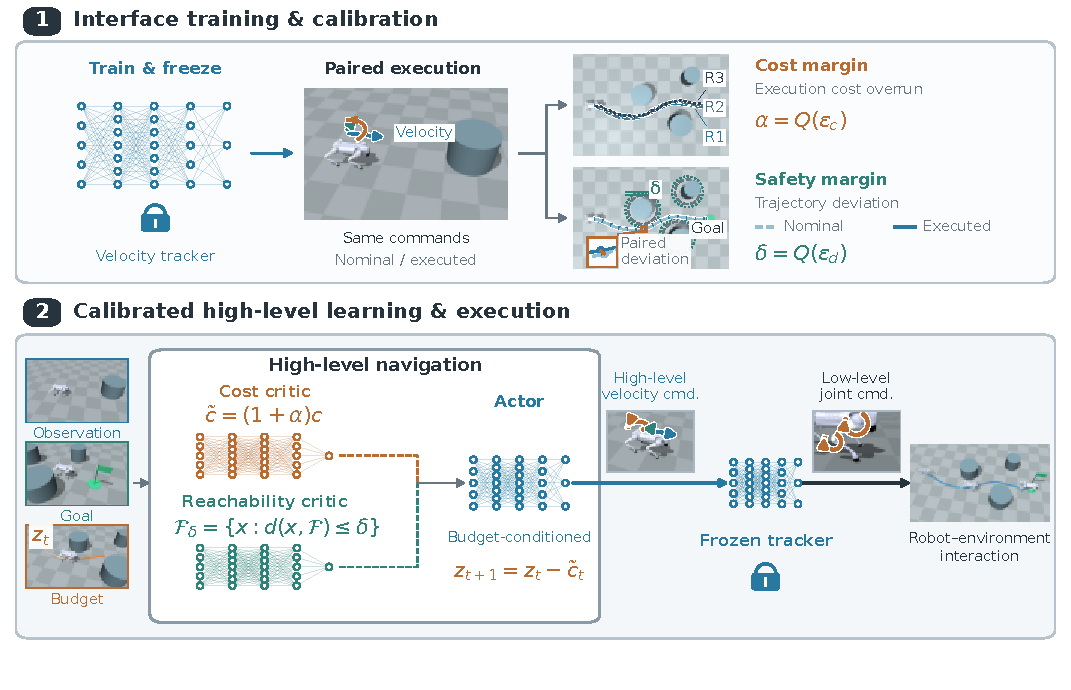
\includegraphics[width=\columnwidth]{../../images/1114/deployment_calibration_overview.pdf}
\caption{CaMRA architecture. In Stage 1, a frozen velocity interface is established
and execution margins are calibrated. In Stage 2, the margins are incorporated into
high-level navigation learning and budget selection, with the same tracker retained for execution.
Scenes and paths are schematic; successive robot states are represented by ghost poses.}
\label{fig:system_overview}
\end{figure}

\subsection{Hierarchical Control with a Frozen Velocity Interface}
Direct joint-level MCRA learning couples stable locomotion with goal reaching,
obstacle avoidance, and cost reduction. Avoiding falls and excessive tilt alone
gives limited guidance for coordinated, smooth locomotion, and early balance
loss can interrupt navigation exploration. Hierarchical control therefore
separates locomotion stabilization from high-level reach-avoid decisions.

The tracker is pretrained with PPO and domain randomization to maintain balance,
gait coordination, and action smoothness while tracking velocity commands.
It maps proprioception and body-velocity commands
$u_t=[v_x^*,v_y^*,\omega_z^*]^\top$ to joint commands, attenuating disturbances
through closed-loop feedback within its trained command domain. Freezing it
before calibration and high-level learning prevents subsequent low-level
parameter changes; the navigation policy learns velocity commands rather than
joint coordination.

The nominal map $\bar f_{\mathrm{cl}}$ integrates commanded body velocities over
each high-level interval under ideal tracking. Contact variation, friction,
actuation latency, and state-estimation errors can cause deviations. Calibration,
high-level learning, and deployment share the frozen tracker and command domain,
providing a consistent basis for residual-error measurement and margin calibration.

\subsection{Execution-Mismatch Calibration}
\label{sec:execution_calibration}
Paired nominal and perturbed-execution rollouts use the frozen interface with
identical initial states, maps, goals, and high-level commands. For length $T$,
let $J_{\rm nom}=\sum_{t=0}^{T-1}c(x_t^{\rm nom},u_t)$ and
$J_{\rm exec}=\sum_{t=0}^{T-1}c(x_t^{\rm exec},u_t)$. Calibration and independent
evaluation use disjoint rollout sets; evaluation data do not select margins.

For $J_{\rm nom}>0$, paired costs give $\varepsilon_c$ as defined in
Section~\ref{sec:problem_setup}. Geometric deviation is the maximum planar
distance between time-aligned base positions,
\begin{equation}
\varepsilon_d=\max_{0\leq t\leq T} \left\|p_t^{\rm exec}-p_t^{\rm nom}\right\|_2,
\label{eq:max_planar_deviation}
\end{equation}
where $p_t$ is the base position.

The errors affect different MCRA constraints and are calibrated separately at
quantile levels $p_c$ and $p_d$:
\begin{equation}
\alpha=Q_{p_c}(\varepsilon_c),\qquad
\delta=Q_{p_d}(\varepsilon_d),
\label{eq:calibration_margins}
\end{equation}
where $Q_p$ is the empirical calibration-sample $p$-quantile. The corrected cost
$\tilde c(x_t,u_t)=(1+\alpha)c(x_t,u_t)$ gives budget updates
$z_{t+1}=z_t-\tilde c(x_t,u_t)$, and the unsafe set becomes
$\mathcal{F}_\delta=\{x:d(x,\mathcal{F})\leq\delta\}$. Both margins are fixed
before high-level learning; empirical coverage depends on the execution
conditions represented in calibration.

\subsection{Robust MCRA Learning and Deployment}
Budget-conditioned navigation learning and initial-budget selection use the
corrected cost and expanded unsafe set, incorporating both margins into decisions
executed through the frozen velocity interface.

In Phase I, $\tilde c$ updates the budget, while $\mathcal{F}_\delta$ determines
the safety indicator and augmented goal. A stochastic actor
$\pi_\theta(u\mid o,y,z)$ uses two critics: $V_h$ evaluates goal reaching and
safety, and $V_c$ estimates corrected cumulative cost over the same stopping
horizon. Normalizing cost by the scene-specific reference budget
$z_{\rm ref}>0$ gives
\begin{equation}
W=\max\{V_h,V_c-z/z_{\rm ref}\}.
\label{eq:combined_residual}
\end{equation}
The actor is optimized to reduce this residual. Thus $\alpha$ modifies cost targets and budget
updates, while $\delta$ modifies reachability targets through the safety indicator.

In Phase II, the actor's mean action defines a deterministic deployment policy;
the actor is fixed and the critics are refitted. Under the calibrated model,
we select the smallest tested initial budget satisfying the prescribed
goal-reaching, collision, and budget-violation criteria.

At deployment, the policy receives navigation observations and remaining budget,
and the frozen tracker executes its body-velocity commands. A parallel nominal
rollout driven by the same commands supplies the calibrated budget-update cost.

\section{Experiments}
% Evaluation: overall performance, calibration mechanisms, budget sensitivity,
% execution perturbations, and hardware deployment.
\subsection{Experimental Setup and Evaluation Protocol}
\label{sec:experimental_setup}
The evaluation covers navigation performance, execution-error calibration, margin
contributions and sensitivity, budget selection, disturbance robustness, and
physical deployment. The planar benchmark assesses high-level velocity-interface
decisions; the hardware study examines quadruped execution.

The benchmark uses moderately cluttered, narrow-passage, and densely obstructed
$8\times8$ m maps. Methods share test maps, navigation observations, command
limits, and the frozen tracker, with matched training interaction budgets and network
widths. The decision interval is 0.2 s and horizon 30 s. Each method has three
policies trained with different seeds: 100 trials per policy and scenario give
300 per scenario and 900 overall. Calibration, training, budget selection, and
final evaluation use separate rollout sets.

Metrics are success rate (SR), mean executed cost (Cost), physical collision rate
(CR), budget violation rate (BVR), and mean per-trial minimum clearance (MC).
Success requires collision-free goal reaching before timeout; budget compliance
is separate. Collision and clearance use a common physical footprint. Cost and
MC include all trials until goal reaching, collision, or timeout; evaluation
continues after budget exceedance. Reference budgets $z_{\rm ref}$ are 120, 140,
and 190 a.u. for the moderately cluttered, narrow-passage, and densely obstructed
scenes, respectively. The ratio $z_0/z_{\rm ref}$ normalizes initial budget.
Tables report equally weighted scene means at $z_0/z_{\rm ref}=1$; scene-level
intervals describe test-case variability conditional on the trained policies.

Baselines are uncalibrated RC-PPO, reach-avoid learning (RA), reward-based proximal
policy optimization (PPO), and constrained PPO (CPPO), all using the same frozen
tracker. Uncalibrated RC-PPO sets both margins to zero. RA retains goal reaching and avoidance
but omits cost minimization and budget input. PPO and CPPO use lower/higher
collision-penalty weights $\beta_L=1$/$\beta_H=5$; CPPO additionally imposes
$\mathbb{E}[J/z_{\rm ref}]\leq1$ on expected cumulative cost.

\subsection{Overall Navigation Performance}
\label{sec:overall_performance}
Table~\ref{tab:main_results} compares overall performance;
Fig.~\ref{fig:metrics_draft} reports the five metrics by scene. Relative to
uncalibrated RC-PPO, CaMRA raises mean SR from 70.7\% to 73.3\%, reduces Cost
from 91.7 to 88.3 a.u. and BVR from 14.0\% to 9.0\%, with similar CR
(15.7\% for RC-PPO versus 15.0\% for CaMRA). RA and CPPO$_{\beta_L}$ achieve lower CR and greater
clearance but lower SR and higher Cost and BVR, illustrating the joint
success--safety--cost trade-off.

\begin{table}[!htbp]
\caption{Equal-scene mean performance at $z_0/z_{\rm ref}=1$.
Cost is interpreted jointly with SR.}
\label{tab:main_results}
\centering
\small
\setlength{\tabcolsep}{3pt}
\renewcommand{\arraystretch}{1.12}
\begin{tabular}{@{}lccccc@{}}
\hline
Method & \shortstack{SR\\(\%) $\uparrow$} & Cost & \shortstack{CR\\(\%) $\downarrow$} & \shortstack{BVR\\(\%) $\downarrow$} & \shortstack{MC\\(m) $\uparrow$}\\
\hline
\rowcolor{methodblue!9}
\textbf{CaMRA} & \textbf{73.3} & \textbf{88.3} & 15.0 & \textbf{9.0} & 0.31\\
RC-PPO & 70.7 & 91.7 & 15.7 & 14.0 & 0.30\\
RA & 60.0 & 104.0 & 13.0 & 20.0 & 0.34\\
PPO$_{\beta_L}$ & 67.7 & 99.7 & 23.0 & 20.7 & 0.20\\
PPO$_{\beta_H}$ & 42.3 & 117.0 & 29.0 & 27.0 & 0.16\\
CPPO$_{\beta_L}$ & 37.7 & 124.7 & \textbf{12.3} & 22.3 & \textbf{0.36}\\
CPPO$_{\beta_H}$ & 69.7 & 105.7 & 18.3 & 17.0 & 0.26\\
\hline
\end{tabular}
\end{table}

\begin{figure}[!htbp]
\centering
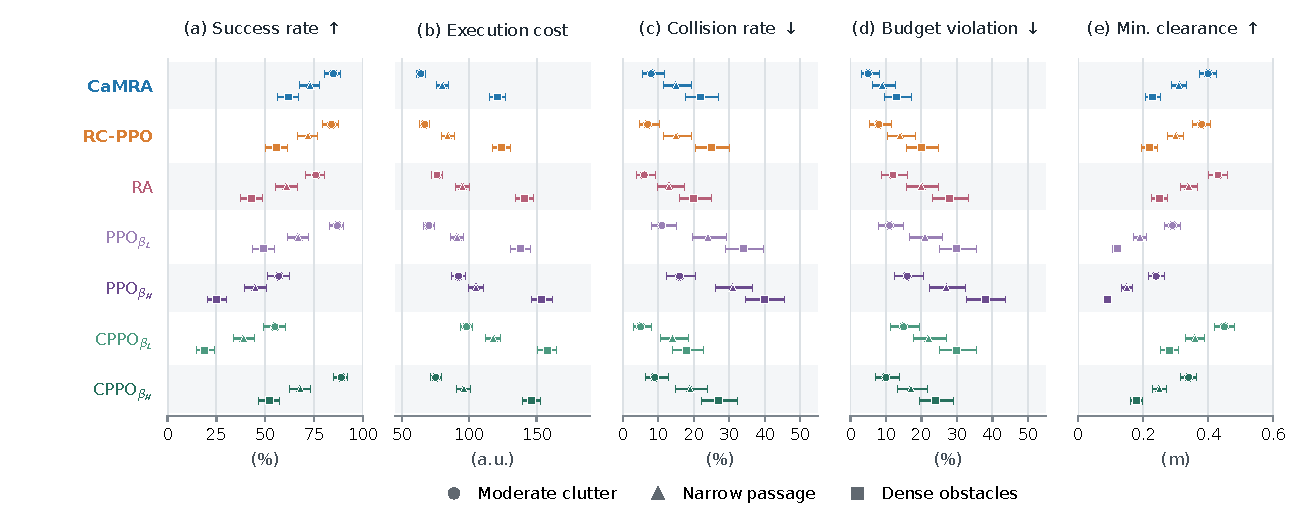
\includegraphics[width=\columnwidth]{../../images/1114/metrics_comparison.pdf}
\caption{Scenario-level SR, Cost, CR, BVR, and MC at the common reference budget.
Scenarios and methods are distinguished by markers and colors, respectively.
Points show the computed metric values; horizontal bars show the corresponding
95\% intervals conditional on the three trained policies ($n=300$ per method and scene). Equal-scene means
are reported in Table~\ref{tab:main_results}.}
\label{fig:metrics_draft}
\end{figure}

In the paired example of Fig.~\ref{fig:trajectory_sync}, CaMRA follows a slightly
longer, costlier route with greater clearance under the geometric margin $\delta$.
Obstacle passages are marked in synchronized clearance, executed-cost, and
tracking-error curves; the corrected nominal charge illustrates $\alpha$'s
budget-accounting role. Both methods satisfy the common budget, illustrating a
safety--cost trade-off. This separate diagnostic uses the same proxy cost and
is excluded from Table~\ref{tab:main_results}.

\begin{figure}[!htbp]
\centering
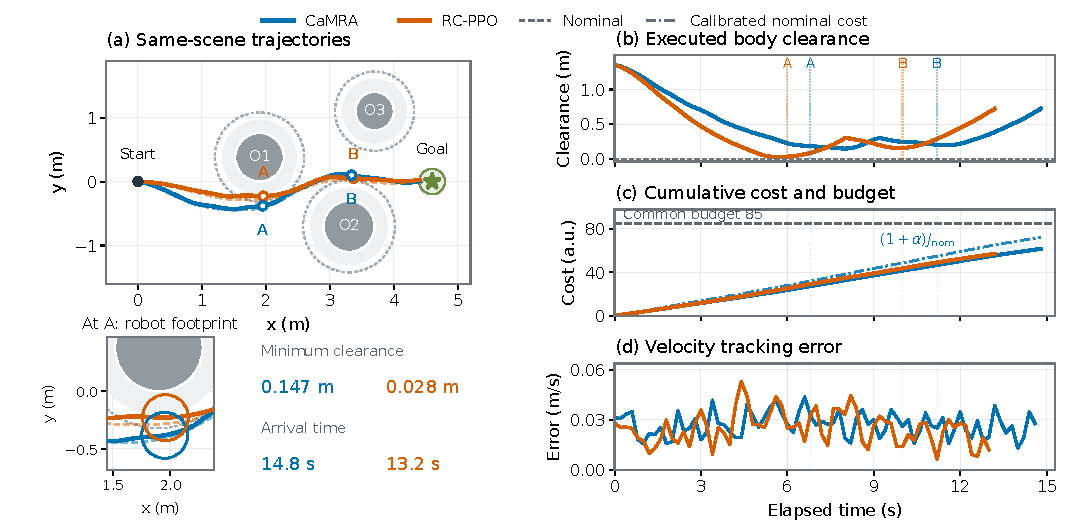
\includegraphics[width=\columnwidth]{../../images/1114/trajectory_sync.pdf}
\caption{Same-scene trajectories and synchronized diagnostics for CaMRA (blue)
and RC-PPO (orange), with a common initial budget of 85 a.u.
(a) Executed (solid) and nominal (dashed) paths, with $\delta=0.12$ m.
(b) Physical clearance. (c) Cumulative costs, budget, and corrected charge
$(1+\alpha)J_{\rm nom}$, with $\alpha=0.18$. (d) Linear-velocity tracking error.
Each method's obstacle passages are marked by A/B; traces are truncated at the
respective terminations.}
\label{fig:trajectory_sync}
\end{figure}

\subsection{Execution-Error Calibration and Margin Analysis}
\label{sec:mismatch_analysis}
Execution mismatch is summarized in Fig.~\ref{fig:margin_calibration} using 800
calibration and 400 held-out paired rollouts. In the calibration set, the medians
are $0.09$ for relative cost overrun and
$0.06$ m for maximum planar position deviation; $\alpha=0.18$ and $\delta=0.12$ m
are set to the respective 90th percentiles. With these margins fixed, held-out
coverage is $353/400$
($88.25\%$) for cost and $346/400$ ($86.50\%$) for position. These marginal
coverages are used to assess the error allowances in budget accounting and obstacle
inflation; joint held-out coverage is $336/400$ ($84.0\%$). Neither marginal nor
joint error coverage is a navigation success probability.

\begin{figure}[!htbp]
\centering
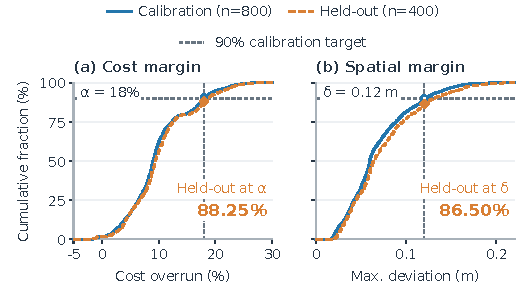
\includegraphics[width=\columnwidth]{../../images/1114/margin_calibration.pdf}
\caption{Execution-error calibration and held-out assessment.
Calibration and held-out empirical CDFs are shown as blue solid and orange dashed
curves. The calibration 90th percentiles and 90\% target are marked by vertical
and horizontal lines, respectively. Coverage at the fixed thresholds, including
ties, is indicated by circles and diamonds.}
\label{fig:margin_calibration}
\end{figure}

Table~\ref{tab:ablation_draft} and Fig.~\ref{fig:ablation_margins} compare margin
ablations with the same frozen tracker. Single-margin variants set $\alpha=0$
or $\delta=0$, retaining the other's calibrated value; removing both recovers
uncalibrated RC-PPO. Without $\alpha$, BVR rises by 13.4 percentage points;
without $\delta$, CR rises by 11.3 percentage points and clearance decreases.

\begin{table}[!htbp]
\caption{Margin ablation with the same frozen tracker and reference budget as
Table~\ref{tab:main_results}.
Cost is interpreted jointly with SR.}
\label{tab:ablation_draft}
\centering
\small
\setlength{\tabcolsep}{3pt}
\renewcommand{\arraystretch}{1.12}
\begin{tabular}{@{}lccccc@{}}
\hline
Variant & \shortstack{SR\\(\%) $\uparrow$} & Cost & \shortstack{CR\\(\%) $\downarrow$} & \shortstack{BVR\\(\%) $\downarrow$} & \shortstack{MC\\(m) $\uparrow$}\\
\hline
\rowcolor{methodblue!9}
\textbf{CaMRA} & \textbf{73.3} & 88.3 & \textbf{15.0} & \textbf{9.0} & \textbf{0.31}\\
w/o both (RC-PPO) & 70.7 & 91.7 & 15.7 & 14.0 & 0.30\\
w/o $\alpha$ & 67.2 & 80.6 & 19.8 & 22.4 & 0.29\\
w/o $\delta$ & 64.8 & \textbf{77.2} & 26.3 & 13.8 & 0.19\\
\hline
\end{tabular}
\end{table}

Full and zero-margin rows reuse the CaMRA and RC-PPO results in
Table~\ref{tab:main_results}. Single-margin variants are trained separately with
the margin removed in both learning and evaluation. Effects are non-additive;
more failures or shorter trajectories can lower Cost, which must be interpreted
jointly with SR.

\begin{figure}[!htbp]
\centering
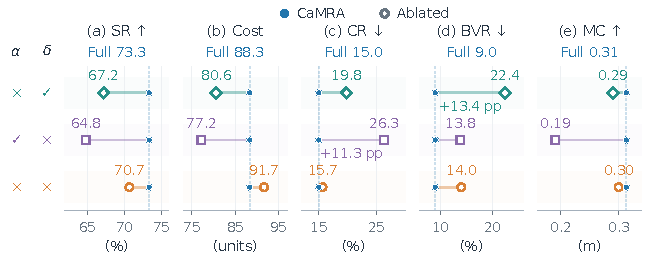
\includegraphics[width=\columnwidth]{../../images/1114/ablation_horizontal.pdf}
\caption{Effects of removing the cost margin $\alpha$ and geometric margin
$\delta$ at the common reference budget. Changes between variants are indicated
by connecting lines.}
\label{fig:ablation_margins}
\end{figure}

To assess margin sensitivity beyond component removal, the high-level networks
are retrained for each of 16 combinations
of $\alpha\in\{0,0.09,0.18,0.27\}$ and
$\delta\in\{0,0.06,0.12,0.18\}$ m, with the frozen tracker, training
budget, and 900-trial evaluation protocol retained. The four zero/calibrated combinations
match Table~\ref{tab:ablation_draft}. With both margins increased to $(0.27,0.18)$,
CR and BVR are reduced to 13.3\% and 6.7\%, but SR is lowered to 68.0\% and
cost is raised to 95.0 a.u. A more conservative trade-off is thus observed as the
margins are increased.
Calibration is performed before the sweep and is not retuned to maximize these
results.

\subsection{Budget Selection and Performance Trade-offs}
\label{sec:budget_sensitivity}
With policy and margins fixed, budget selection uses separate rollouts, while
Fig.~\ref{fig:budget_draft} shows final-evaluation budget responses. RA reuses
the same trajectories at every threshold, so only BVR changes. Under SR
$\geq60\%$, CR $\leq20\%$, and BVR $\leq15\%$, the smallest tested ratios
satisfying all criteria on the final curves are $0.90$ for CaMRA, $0.96$ for
RC-PPO, and $1.12$ for RA. CaMRA thus meets the same criteria at a lower tested
budget.
\begin{figure}[!htbp]
\centering
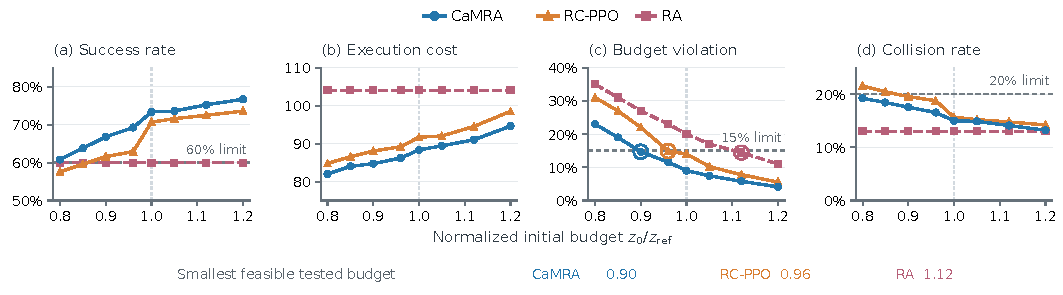
\includegraphics[width=\columnwidth]{../../images/1114/budget_sweep_horizontal.pdf}
\caption{Budget-response curves averaged equally across scenarios. Acceptance
thresholds are indicated by dashed lines; the smallest tested budgets satisfying
all three criteria are marked by outlined points. Results at the reference budget match
Table~\ref{tab:main_results}.}
\label{fig:budget_draft}
\end{figure}

\subsection{Robustness to Execution Perturbations}
\label{sec:execution_robustness}
With the policy and margins fixed, performance is evaluated under execution
conditions that differ from those used for calibration. Each profile's deviation
from the nominal condition is increased by 25\%: the minimum friction is
0.4875, the maximum delay is 0.125 s, and the maximum
velocity-noise standard deviation is 0.05 m/s. Across 900 independent
trials (60 per profile and scene), SR is
$65.0\%$ and BVR $16.0\%$ for CaMRA versus SR $58.0\%$ and BVR $24.0\%$ for
uncalibrated RC-PPO. The corresponding CR values are 22.0\% and 27.0\%, costs
are 96.8 and 102.4 a.u., and MC values are 0.26 and 0.24 m. No policy or margin
is refitted for this stress test. Under the tested perturbations, higher success
and lower collision and budget-violation rates are obtained with CaMRA than with
uncalibrated RC-PPO.

\subsection{Physical-Robot Deployment and Failure Analysis}
\label{sec:hardware_deployment}
A Unitree Go2 is evaluated in two cluttered indoor settings:
Fig.~\ref{fig:hardware_sequences}(a) examines collision avoidance in an
obstacle-filled corridor; Fig.~\ref{fig:hardware_sequences}(b) examines low-cost
route selection among multiple chair-obstacle passages.

\begin{figure}[!htbp]
\centering
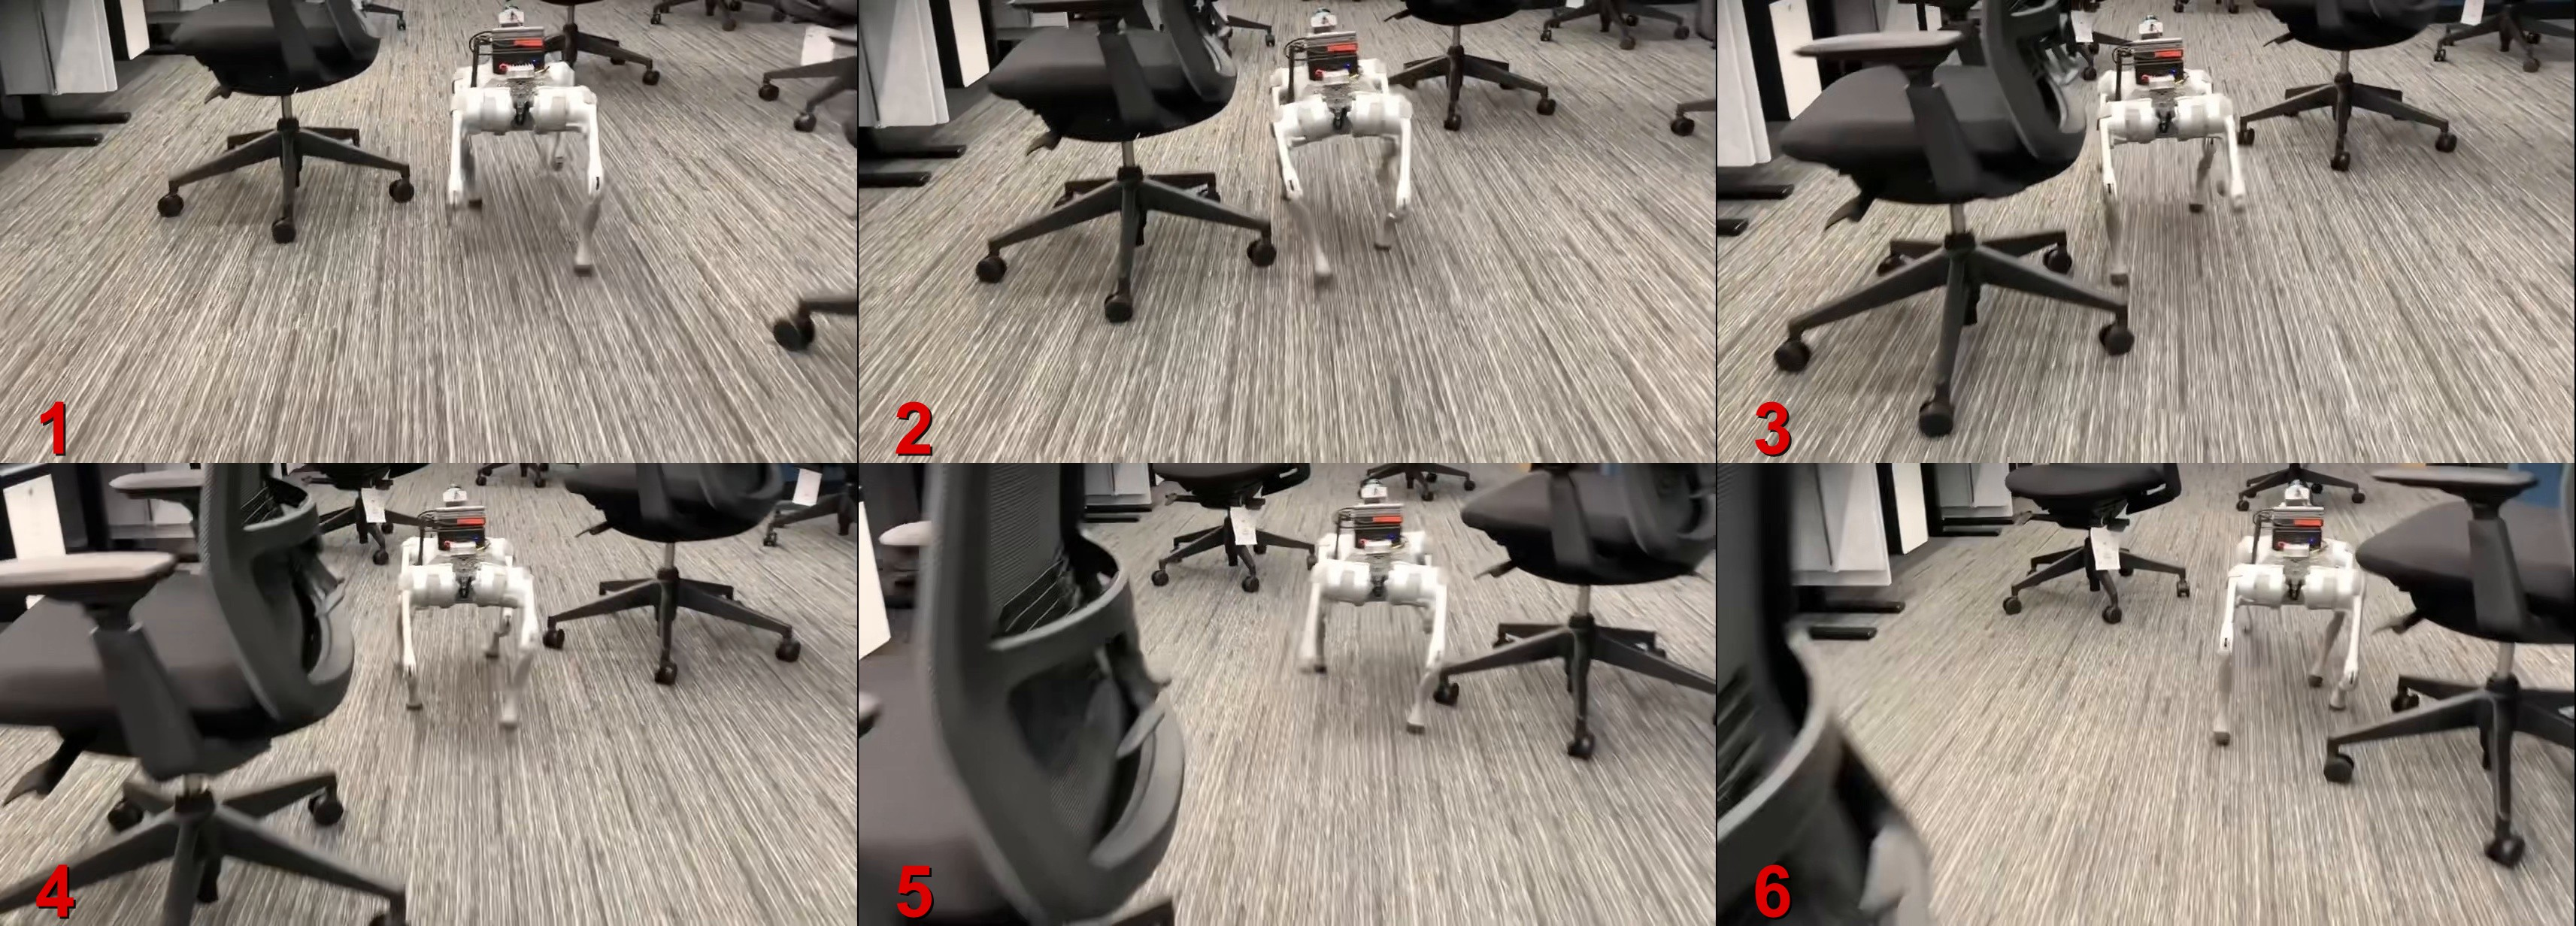
\includegraphics[width=\columnwidth]{../../images/1114/office_sequence_candidate_A_numbered.jpg}
\par\smallskip
{\footnotesize (a) Obstacle avoidance in a cluttered corridor.\par}
\medskip
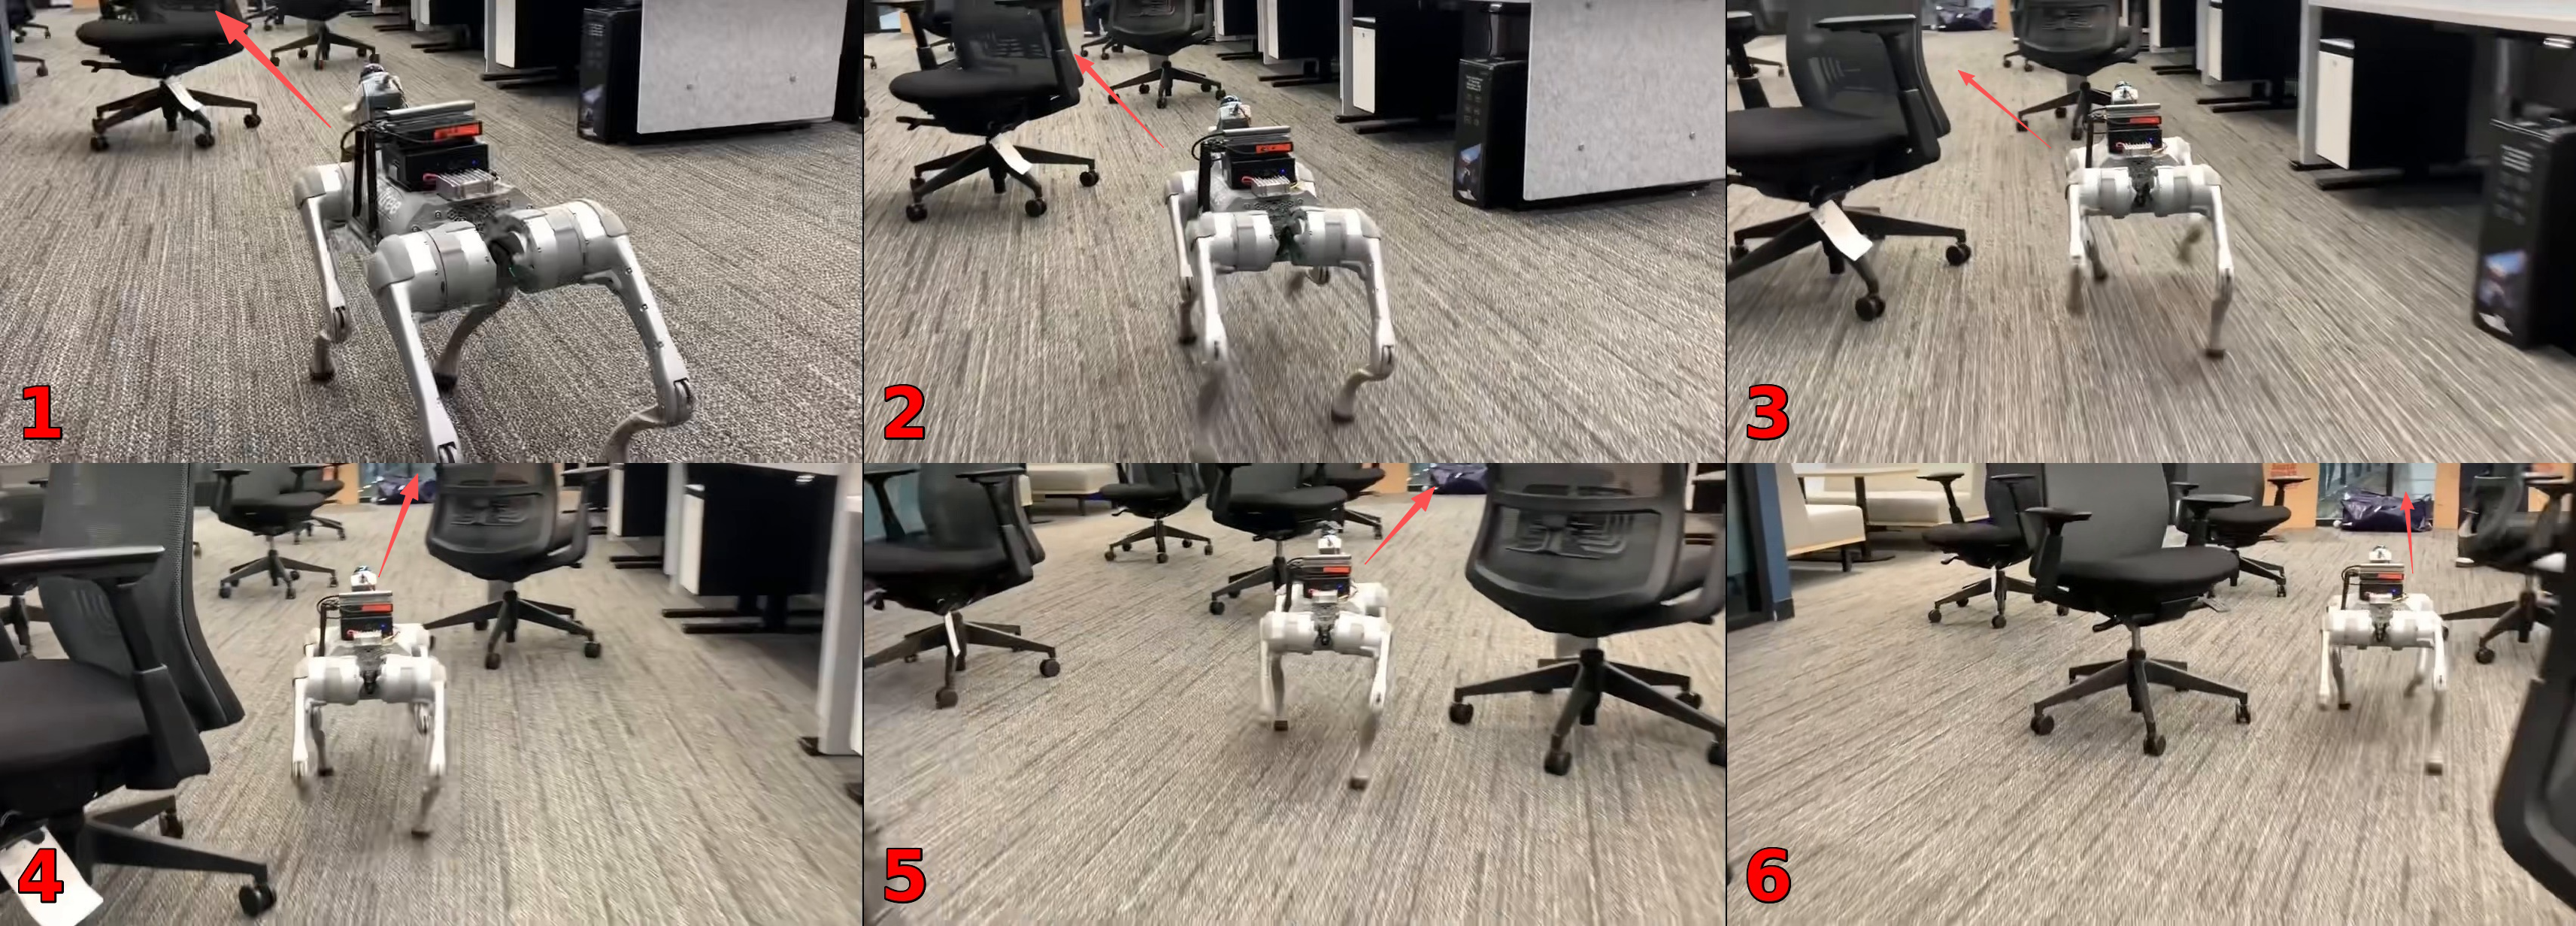
\includegraphics[width=\columnwidth]{../../images/1114/office_shortest_path_sequence_final.png}
\par\smallskip
{\footnotesize (b) Low-cost route selection among chair obstacles.\par}
\caption{Physical deployment of Unitree Go2: (a) corridor traversal with obstacle
avoidance; (b) route selection among multiple passages formed by chairs. Each
panel comprises six successive frames in temporal order; the travel direction
is indicated by red arrows in (b).}
\label{fig:hardware_sequences}
\end{figure}

The representative route is approximately 15 m long and includes a narrow
passage about 0.3 m wider than the robot body. Proprioceptive measurements are
provided by joint encoders and the IMU; navigation observations are obtained from
projected LiDAR ranges and local scan matching.
Policies are executed on an onboard x86-64 CPU with 16 GB RAM, at the same
50 Hz/5 Hz control rates. A 60 s horizon and a budget of 230 a.u. are used for the
15 m task; the tracker, navigation policy, and margins are held fixed.

Table~\ref{tab:hardware_comparison} compares CaMRA and uncalibrated RC-PPO with
matched scenes, starts, goals, and budget. Both share the frozen tracker and
navigation inputs; high-level policies remain fixed throughout evaluation.

\begin{table}[!htbp]
\caption{Hardware performance comparison with 50 trials per method.
Cost is in a.u. and is interpreted jointly with SR.}
\label{tab:hardware_comparison}
\centering
\small
\setlength{\tabcolsep}{3pt}
\renewcommand{\arraystretch}{1.12}
\begin{tabular}{@{}lccccc@{}}
\hline
Method & \shortstack{SR\\(\%) $\uparrow$} & Cost & \shortstack{CR\\(\%) $\downarrow$} & \shortstack{BVR\\(\%) $\downarrow$} & \shortstack{MC\\(m) $\uparrow$}\\
\hline
\rowcolor{methodblue!9}
\textbf{CaMRA} & \textbf{70.0} & 182.0 & \textbf{16.0} & \textbf{14.0} & \textbf{0.09}\\
RC-PPO & 64.0 & \textbf{176.0} & 20.0 & 22.0 & 0.07\\
\hline
\end{tabular}
\end{table}

CaMRA succeeds in $35/50$ trials versus $32/50$ for RC-PPO. Both have three
localization aborts; remaining failures are four timeouts and eight contacts for
CaMRA, versus five timeouts and ten contacts for RC-PPO. BVR decreases from
22.0\% to 14.0\%, while mean cost increases from 176.0 to 182.0 a.u. These
results indicate a clearance--cost trade-off: shorter routes and earlier failures
can lower mean cost without reducing its upper tail. Cost and MC include all
terminal outcomes. Hardware results are separate from the planar benchmark
because route, horizon, and footprint differ.

\section{Conclusion}
CaMRA connects quadruped MCRA navigation to execution through hierarchical control
and calibration. A frozen low-level controller stabilizes motion while a
high-level policy learns navigation, mitigating coupled learning. Separate cost
and geometric margins account for residual nominal/execution mismatch. The
evaluations illustrate their effects on budget compliance, obstacle clearance,
and goal reachability. Future work will explore semantic task understanding and
stochastic formulations in which execution uncertainty can be incorporated into
formal reach-avoid and cost guarantees.

% Activate balancing within the first column of the reference page.
\IEEEtriggeratref{1}
\IEEEtriggercmd{\balance}
\bibliographystyle{IEEEtran}
\bibliography{references}

\end{document}
